\documentclass[notheorems,aspectratio=169]{beamer}

\author{Владислав Шаршуков}
\date{\today}
\title{Робастность дискретных систем}

%% \usetheme{Warsaw}
\usetheme{default}
\usefonttheme{serif}

\usepackage[utf8]{inputenc}
\usepackage[T2A]{fontenc}
\usepackage[russian]{babel}
\usepackage{graphicx}
\usepackage{longtable}
\usepackage{wrapfig}
\usepackage{rotating}
\usepackage[normalem]{ulem}
\usepackage[makeroom]{cancel}
\usepackage{amsmath}
\usepackage{amssymb}
\usepackage{capt-of}
\usepackage{hyperref}

\usepackage[backend=biber]{biblatex}

\graphicspath{ {./Images/} }

\addbibresource{DiscreteRobustness.bib}

\theoremstyle{definition}
\newtheorem{theorem}{Теорема}
\newtheorem{definition}{Определение}
\newtheorem{remark}{Замечание}
\newtheorem{proposition}{Утверждение}
\newtheorem{lemma}[theorem]{Лемма}
\newtheorem{corollary}[theorem]{Следствие}
\newtheorem{solution}{Решение} % FIXME: solution is not a theorem

\newcommand{\highlight}[1]{{\color{red} #1}}
\newcommand{\abs}[1]{\left| #1 \right|}
\newcommand{\paren}[1]{\left(#1\right)}
\renewcommand{\emph}[1]{\uline{#1}}
\renewcommand{\Re}{\operatorname{Re}}
\renewcommand{\Im}{\operatorname{Im}}

\setbeamertemplate{section in toc}[sections numbered]
\setbeamertemplate{footline}{}
\setbeamertemplate{headline}{}
\setbeamertemplate{navigation symbols}{}

%% ================================== %%

\begin{document}

\begin{frame}
  \titlepage{}
\end{frame}

\begin{frame}{Содержание}
  \tableofcontents
\end{frame}

\section{Дискретные системы. Введение, устойчивость}

\begin{frame}{Разностное уравнение. $z$-преобразование}
  Разностное уравнение (в обратных разностях):
  \begin{equation*}
    \nabla^N y(n) + \alpha_1 \nabla^{N-1} y(n) + \cdots + \alpha_N y(n) = 
    \beta_0 \nabla^M x(n) + \beta_1 \nabla^{M-1} x(n) + \cdots + \beta_M x(n).
  \end{equation*}

  $z$-преобразование:
  \begin{equation*}
    Z\left\{ f(n) \right\} = F(z) = \sum_{n=0}^\infty f(n) z^{-n}.
  \end{equation*}

  Таблицу $z$-преобразований можно найти в~\cite[с.~255]{Kargu1974}.
\end{frame}

\begin{frame}{Передаточная функция. Характеристический полином}
  \begin{definition}
    \textit{Передаточной функцией} разностной системы называют отношение
    $z$-преобразования выходной последовательности $y(n)$ к $z$-преобразованию
    входной последовательности $x(n)$ при нулевых начальных условиях:
    \begin{equation*}
      \Phi(z) = \frac{Z\left\{ y(n) \right\}}{Z\left\{ x(n)\right\}} = \frac{Y(z)}{X(z)}.
    \end{equation*}
  \end{definition}

  \begin{definition}
    Знаменатель передаточной функции $X(z)$ называют \textit{характеристическим полиномом} разностного уравнения.
  \end{definition}
\end{frame}

\begin{frame}{Пример}
  Разностное уравнение:
  \begin{equation*}
    y(n) + (\alpha - 1) y(n - 1) = \alpha x(n), \quad 0 < \alpha < 1.
  \end{equation*}
  Применим $z$-преобразование при нулевых начальных данных ($y(-1) = 0$):
  \begin{equation*}
    Y(z) + (\alpha - 1) z^{-1} Y(z) = \alpha X(z).
  \end{equation*}
  Передаточная функция:
  \begin{equation*}
    \Phi(z) = \frac{Y(z)}{X(z)} = \frac{\alpha}{1 + (\alpha - 1) z^{-1}} = \frac{\alpha z}{z + (\alpha - 1)}.
  \end{equation*}

  Характеристический полином: $z + (\alpha - 1)$.
\end{frame}

\begin{frame}{Область устойчивости дискретной системы}
  Характеристический полином системы:
  \begin{equation*}
    a(z) = a_0 z^m + a_1 z^{m-1} + \cdots + a_m = a_0 \prod_{i=1}^m (z - z_i).
  \end{equation*}

  \begin{proposition}[{\cite[с.~259]{Kargu1974}}]
    Для устойчивости дискретной системы необходимо, чтобы корни её характеристического полинома
    $a(z)$ лежали внутри единичной окружности:
    \begin{equation*}
      \abs{z_i} < 1 \quad \forall i=\overline{1,m}.
    \end{equation*}
  \end{proposition}
\end{frame}

\begin{frame}{Скрытая неустойчивость}
  \begin{remark}
    Условие $\abs{z_i} < 1, \; \forall i=\overline{1,m}$ гарантирует устойчивость только в дискретные моменты времени,
    поэтому возможны случаи ``скрытой'' неустойчивости, когда $y(n)$ затухает, а $y(t)$ не затухает или расходится:
    \begin{center}
      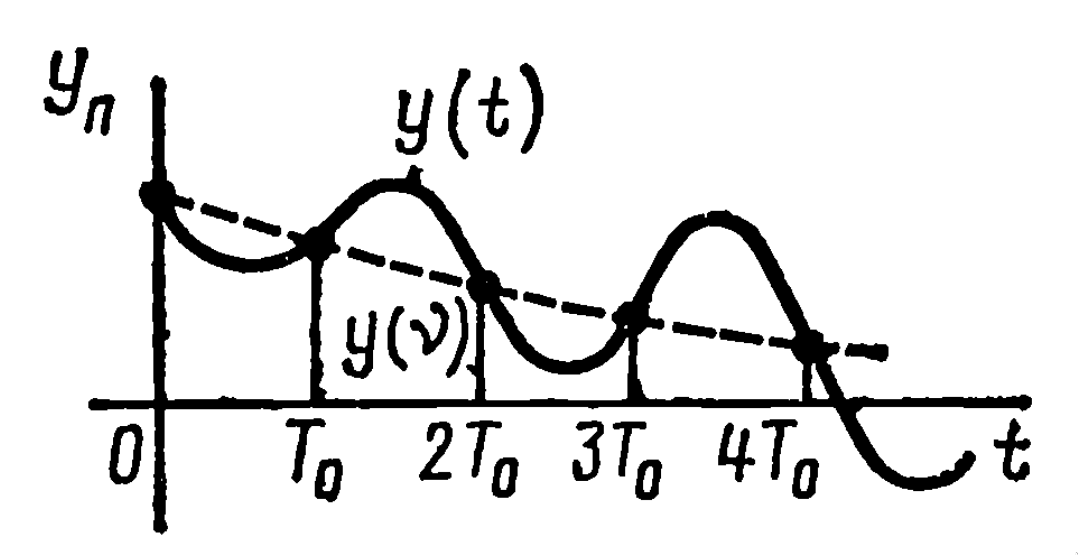
\includegraphics[width=8cm]{HiddenInstability}
    \end{center}
  \end{remark}
\end{frame}

\begin{frame}{Билинейное преобразование}
  \begin{proposition}[{\cite[с.~1214]{KrausAndersonMansour1988}}]
    Если все корни полинома $f(z)$ лежат в единичной окружности, то все корни полинома
    \begin{equation*}
      g(s) = {(s - 1)}^n f\paren{\frac{s+1}{s-1}}
    \end{equation*}
    лежат в левой полуплоскости $\Re{s} < 0$.
  \end{proposition}
\end{frame}

\section{Теоремы Харитонова. Неприменимость в дискретном случае}

\begin{frame}{Интервальный полином}
  \begin{definition}
    \textit{Интервальным полиномом} называется семейство полиномов
    \begin{equation}\label{def:interval-polynomial}
      F(s) = \sum_{k=0}^n a_k s^k,
      \quad a_k \in [\underline{a}_k, \overline{a}_k],
      \quad \underline{a}_k \leqslant \overline{a}_k
      \quad \forall k=\overline{0,n}
    \end{equation}
  \end{definition}

  \begin{definition}
    \textit{Угловыми полиномами} называются полиномы вида~\eqref{def:interval-polynomial},
    где либо \(a_k = \underline{a}_k\), либо
    \(a_k = \overline{a}_k\) для всех \(k=\overline{1,n}\).
  \end{definition}
\end{frame}

\begin{frame}{Теоремы Харитонова}
  \begin{theorem}[Харитонова, слабая]
    Необходимым и достаточным условием робастной устойчивости интервального
    полинома является гурвицевость всех его угловых полиномов.
  \end{theorem}

  \begin{theorem}[Харитонова, сильная]
    Необходимым и достаточным условием робастной устойчивости интервального
    полинома является гурвицевость лишь четырёх полиномов:

    \begin{equation}
      \begin{aligned}
        F_1(s) &= \underline{a}_0 + \overline{a}_1 s + \overline{a}_2 s^2 +
        \underline{a}_3 s^3 + \underline{a}_4 s^4 + \dots \\
        F_2(s) &= \underline{a}_0 + \underline{a}_1 s + \overline{a}_2 s^2 +
        \overline{a}_3 s^3 + \underline{a}_4 s^4 + \dots \\
        F_3(s) &= \overline{a}_0 + \underline{a}_1 s + \underline{a}_2 s^2 +
        \overline{a}_3 s^3 + \overline{a}_4 s^4 + \dots \\
        F_4(s) &= \overline{a}_0 + \overline{a}_1 s + \underline{a}_2 s^2 +
        \underline{a}_3 s^3 + \overline{a}_4 s^4 + \dots
      \end{aligned}
    \end{equation}
  \end{theorem}
\end{frame}

\begin{frame}{Контрпример для дискретного случая}
  Рассмотрим многочлен
  \begin{equation}
    g(b_1, z) = z^4 + b_1z^3 + \frac{3}{2} z^2 - \frac{1}{3}, \quad b_1 \in \left[\frac{-17}{8}, \frac{17}{8}\right].
  \end{equation}

  Полиномы $g(-17/8, z)$ и $g(17/8, z)$ являются полиномами Шура, а $g(0, z)$ -- нет.
\end{frame}

\begin{frame}{Трудности применения билинейного преобразования}
  Матрица билинейного преобразования неортогональна, следовательно, преобразование
  не сохраняет \textit{прямоугольность} области изменения коэффициентов характеристического полинома $f(z)$ дискретной системы.
\end{frame}

\begin{frame}{Пример}
  Характеристический полином: $f(z) = az^2, \quad a \in [1, 2]$.

  Применяем билинейное преобразование:
  \begin{equation*}
    \begin{aligned}
      g(s) &= {(s-1)}^n f\paren{\frac{s+1}{s-1}} \\
      &= \cancel{{(s - 1)}^2} \cdot a \frac{{(s + 1)}^2}{\cancel{{(s - 1)}^2}} \\
      &= as^2 + 2as + a.
    \end{aligned}
  \end{equation*}

  Область изменения коэффициентов многочлена $g(s)$ непрямоугольна, поэтому теорема Харитонова неприменима.
\end{frame}

\section{Дискретный аналог: слабая теорема Харитонова}

\begin{frame}{Аналог, вариант, эквивалент~\cite{JuryMansour1985}}
  \begin{itemize}
  \item \textit{Дискретный \emph{аналог} критерия} --- критерий в дискретном случае по \emph{форме}
    совпадает с критерием в непрерывном случае
  \item \textit{Дискретный \emph{вариант} критерия} --- критерий в дискретном случае по \emph{сути}
    совпадает с критерием в непрерывном случае
  \item \textit{Дискретный \emph{эквивалент} критерия} --- критерий в дискретном случае по \emph{форме} и \emph{сути}
    совпадает с критерием в непрерывном случае

  \end{itemize}
\end{frame}

\begin{frame}{Вспомогательные определения}
  Рассмотрим полином
  \begin{equation*}
    D(z) = d_0 + d_1 z + \cdots + d_n z^n.
  \end{equation*}

  Введём обозначение:
  \begin{equation*}
    D^*(z) = z^n D(z^{-1}) = d_0 z^n + d_1 z^{n-1} + \cdots + d_n.
  \end{equation*}

  \begin{definition}
    Полином $S(z)$ называется \textit{симметричным}, если $S^*(z) = S(z)$.
  \end{definition}

  \begin{definition}
    Полином $A(z)$ называется \textit{антисимметричным}, если $A^*(z) = -A(z)$.
  \end{definition}
\end{frame}

\begin{frame}{Вспомогательные определения}
  \begin{proposition}[{\cite{Bistritz1984}}]
    Любой многочлен $D_k(z)$ степени $k$ с вещественными коэффициентами
    может быть записан как сумма симметричного и антисимметричного многочленов:

    \begin{equation*}
      D_k(z) = S_k(z) + A_k(z),
    \end{equation*}
    где
    \begin{equation*}
      \begin{aligned}
        S_k(z) &= \frac{1}{2} \left[ D_k(z) + D_k^*(z) \right] \\
        A_k(z) &= \frac{1}{2} \left[ D_k(z) - D_k^*(z) \right]
      \end{aligned}
    \end{equation*}
  \end{proposition}

  \begin{proof}
    Утверждение проверяется непосредственной подстановкой.
  \end{proof}
\end{frame}

\begin{frame}{Демонстрация подхода}
  Рассмотрим многочлен
  \begin{equation*}
    F(z) = \sum_{i=0}^n a_{i} z^i = a_0 \prod_{i=0}^n \paren{z - z_i}, \quad a_i \in \mathbb{R}.
  \end{equation*}

  Определим его симметричную и антисимметричную части:
  \begin{equation*}
    F(z) = F_1(z) + F_2(z),
  \end{equation*}
  где
  \begin{equation*}
    \begin{aligned}
      F_1(z) &= \frac{1}{2} \left[ F(z) + F^*(z) \right] \\
      F_2(z) &= \frac{1}{2} \left[ F(z) - F^*(z) \right] \\
    \end{aligned}
  \end{equation*}
\end{frame}

\begin{frame}{Демонстрация подхода: теорема}
  \begin{theorem}[{\cite{Gnanasekaran1981,Schussler1976}}]
    Полином $F(z)$ устойчив тогда и только тогда, когда выполняются условия:
    \begin{enumerate}
    \item Корни полиномов $F_1(z)$ и $F_2(z)$ лежат на единичной окружности;
    \item Они простые;
    \item Они перемежаются;
    \item $\abs{\dfrac{a_0}{a_n}} < 1$.
    \end{enumerate}
  \end{theorem}

\end{frame}

\begin{frame}{Эквивалентные условия}
  Условия 1-4 эквивалентны следующим:
  \begin{enumerate}
  \item Полюсы и нули функции $\Phi(z) := \dfrac{F_1(z)}{F_2(z)}$ простые, лежащие на единичной окружности;
  \item Если полюс функции $\Phi(z)$ находится в точке $e^{j\psi_k}$, то угол остатка $\Phi(z)$ равен $\psi_k$;
  \item Производная мнимой части функции $\Phi(z)$ по $\varphi$ на единичной окружности положительна:
    \begin{equation*}
      \left. \frac{\partial \Im\left\{ \Phi(z) \right\}}{\partial \varphi} \right|_{r=1} > 0,
    \end{equation*}
  \end{enumerate}

  \begin{remark}
    Условия справедливы и для функции $\Phi^{-1}(z) = \dfrac{F_2(z)}{F_1(z)}$.
  \end{remark}
\end{frame}

\begin{frame}{Доказательство: необходимость}
  \begin{enumerate}
  \item Если корни $F(z)$ лежат внутри единичной окружности, то корни $F^*(z)$ будут лежать снаружи. Сравнивая множители
    $(z - z_i)$ в $F(z)$ и $z(z^{-1} - z_i)$ в $F^*(z)$, найдём, что
    \begin{equation}\label{eq:relations_1}
      \begin{cases}
        \abs{F(z)} < \abs{F^*(z)}, & \abs{z} < 1 \\
        \abs{F(z)} = \abs{F^*(z)}, & \abs{z} = 1 \\
        \abs{F(z)} > \abs{F^*(z)}, & \abs{z} > 1.
      \end{cases}
    \end{equation}
    Введём обозначение
    \begin{equation*}
      Q(z) = \frac{F(z)}{F^*(z)};
    \end{equation*}
    тогда условия перепишутся в виде
    \begin{equation}\label{eq:relations_2}
      \begin{cases}
        \abs{Q(z)} < 1, & \abs{z} < 1, \\
        \abs{Q(z)} = 1, & \abs{z} = 1, \\
        \abs{Q(z)} > 1, & \abs{z} > 1.
      \end{cases}
    \end{equation}
  \end{enumerate}
\end{frame}

\begin{frame}{Доказательство: необходимость}
  \begin{enumerate}
    \setcounter{enumi}{1}
  \item Введём обозначение:
    \begin{equation*}
      \Phi(z) = \frac{F(z) + F^*(z)}{F(z) - F^*(z)} = \frac{F_1(z)}{F_2(z)} = \frac{Q(z) + 1}{Q(z) - 1}.
    \end{equation*}
    Тогда из условий~\eqref{eq:relations_2} следует, что
    \begin{equation}\label{eq:relations_3}
      \Re \left\{ \Phi(z) \right\} = \frac{\abs{Q(z)}^2 - 1}{\abs{Q(z) - 1}^2}
      \begin{cases}
        < 0, & \abs{z} < 1, \\
        = 0, & \abs{z} = 1, \\
        > 0, & \abs{z} > 1.
      \end{cases}
    \end{equation}
  \end{enumerate}
\end{frame}

\begin{frame}{Доказательство: необходимость}
  \begin{enumerate}
    \setcounter{enumi}{2}
  \item Если $z = z_k = \abs{z_k} e^{j \psi_k}$ --- полюс порядка $m$ функции $\Phi(z)$, то для всех достаточно близких $z$
    \begin{equation*}
      \Phi(z) \approx \frac{R_{km}}{{(z - z_k)}^m} = \frac{\abs{R_{km}}}{\rho^m} e^{j (-m\alpha + \beta_k)},
    \end{equation*}
    где $R_{km} = \abs{R_{km}} e^{j \beta_k}$, $z - z_k = \rho e^{j\alpha}$, $\rho$ достаточно мал и $0 \leqslant \alpha \leqslant 2\pi$.
    Отсюда
    \begin{equation*}
      \Re \left\{ \Phi(z) \right\} \approx \frac{\abs{R_{km}}}{\rho^m} \cos\paren{m \alpha - \beta_k}.
    \end{equation*}
    Знак $\Re \left\{ \Phi(z) \right\}$ определяется знаком $\cos\paren{m \alpha - \beta_k}$, изменяющимся $2m$ раз
    при изменении $\alpha$ от $0$ до $2\pi$.
  \end{enumerate}
\end{frame}

\begin{frame}{Доказательство: необходимость}
  \begin{center}
    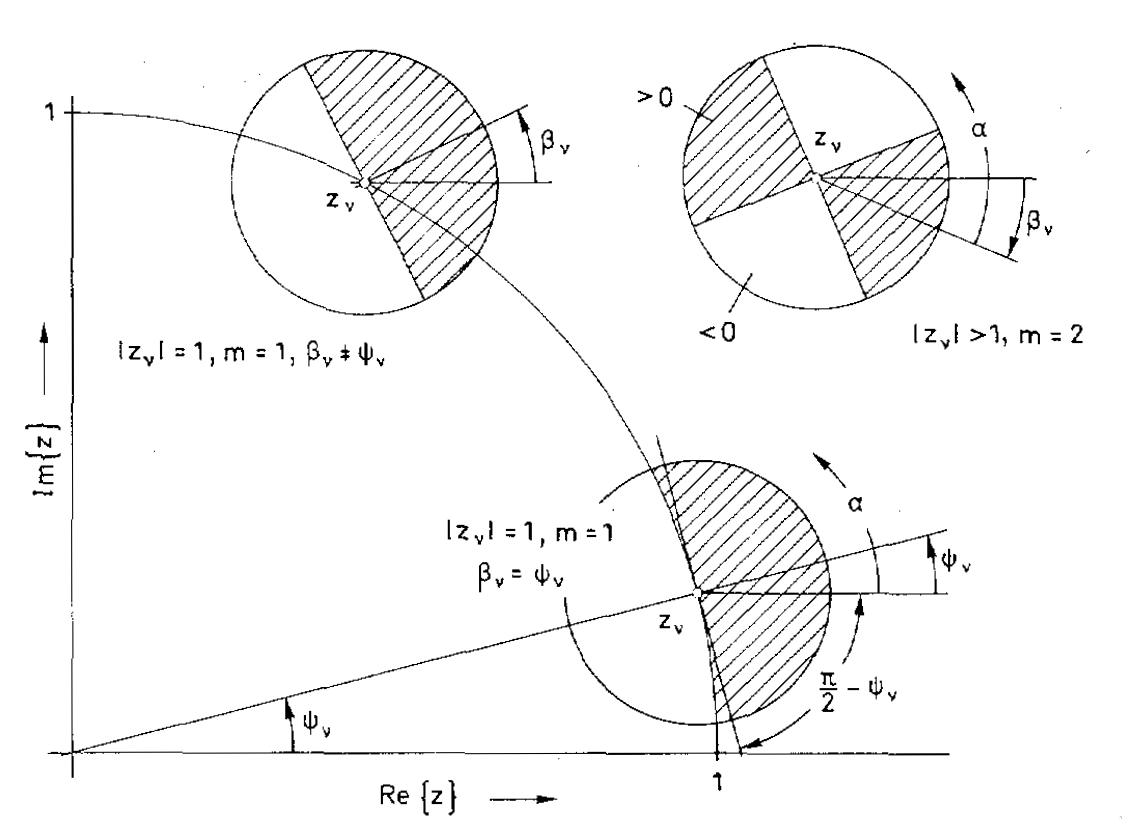
\includegraphics[width=6cm]{Poles}
  \end{center}

  Из~\eqref{eq:relations_3} следует, что знак $\Re \left\{ \Phi(z) \right\}$
  может измениться только на пересечении с единичной окружностью, что влечёт за собой
  условия
  \begin{equation}
    \abs{z_k} = 1, \quad m = 1,
  \end{equation}
  т.е. полюсы функции $\Phi(z)$ простые, лежащие на единичной окружности.
\end{frame}

\begin{frame}{Доказательство: необходимость}
  Следовательно, для достаточно малых $\rho$,
  \begin{equation*}
    \Re \left\{\Phi(z)\right\} \approx \frac{\abs{R_{k}}}{\rho} \cos\paren{\alpha - \beta_k},
  \end{equation*}
  причём
  \begin{equation*}
    \Re \left\{ \Phi(z) \right\} > 0 \quad \mbox{ для } -\frac{\pi}{2} < \paren{\alpha - \beta_k} < \frac{\pi}{2}.
  \end{equation*}
  Знак $\Re \left\{ \Phi(z) \right\}$ изменяется только на пересечении с единичной окружностью, поэтому
  \begin{equation*}
    \Re \left\{ \Phi(z) \right\} > 0 \quad \mbox{ для } -\paren{\frac{\pi}{2} - \psi_k} < \alpha < \frac{\pi}{2} + \psi_k.
  \end{equation*}
  Отсюда $\beta_k = \psi_k$.

  Аналогичный результат достигается для $\dfrac{1}{\Phi(z)}$.
\end{frame}

\begin{frame}{Доказательство: необходимость}
  \begin{enumerate}
    \setcounter{enumi}{3}
  \item Покажем перемежаемость корней $F_1(z)$ и $F_2(z)$.

    В соответствии с~\eqref{eq:relations_3} для $z = r \cdot e^{j\varphi}$
    \begin{equation*}
      \left. \frac{\partial \Re \left\{ \Phi(z) \right\}}{\partial r} \right|_{r=1} > 0.
    \end{equation*}

    Из условий Коши-Римана в полярных координатах следует, что
    \begin{equation*}
      \frac{\partial \Re \left\{ \Phi(z) \right\}}{\partial r} = \frac{1}{r} \frac{\partial \Im\left\{ \Phi(z) \right\}}{\partial \varphi},
    \end{equation*}
    откуда
    \begin{equation*}
      \left. \frac{\partial \Im\left\{ \Phi(z) \right\}}{\partial \varphi} \right|_{r=1} > 0,
    \end{equation*}
    что и влечёт за собой перемежаемость корней. Необходимость доказана.
  \end{enumerate}
\end{frame}

\begin{frame}{Доказательство: достаточность}
  Разложим $\Phi(z)$ на сумму дробей:
  \begin{equation*}
    \Phi(z) = \frac{d_n^{(1)}}{d_n^{(2)}} + \sum_{k=1}^n \frac{\abs{R_k} e^{j \psi_k}}{z - e^{j \psi_k}},
  \end{equation*}
  где
  \begin{itemize}
  \item $d_i^{(1)} = \frac{1}{2}\paren{a_i + a_{n - i}}$ --- коэффициенты $F_1(z)$,
  \item $d_i^{(2)} = \frac{1}{2}\paren{a_i - a_{n - i}}$ --- коэффициенты $F_2(z)$.
  \end{itemize}
\end{frame}

\begin{frame}{Доказательство: достаточность}
  Из симметричности и антисимметричности $F_1(z)$ и $F_2(z)$ следует, что $d_0^{(1)} = d_n^{(1)}$ и $d_0^{(2)} = -d_n^{(2)}$,
  поэтому
  \begin{equation*}
    \Phi(0) = \frac{d_0^{(1)}}{d_0^{(2)}} = -\frac{d_n^{(1)}}{d_n^{(2)}} = \frac{d_n^{(1)}}{d_n^{(2)}} - \sum_{k=1}^n \abs{R_k},
  \end{equation*}
  откуда
 \begin{equation*}
    \sum_{k=1}^n \abs{R_k} = 2 \frac{d_n^{(1)}}{d_n^{(2)}}.
  \end{equation*}
\end{frame}

\begin{frame}{Доказательство: достаточность}
  Достаточность выполнена, если
  \begin{equation}
    \Phi_k(z) = \frac{\abs{R_k} e^{j\psi_k}}{z - e^{j\psi_k}} + b_k
  \end{equation}
  удовлетворяют условию~\eqref{eq:relations_3} при всех $k=\overline{1,n}$.

  Здесь $b_k$ --- положительные вещественные числа, выбранные так, что
  \begin{equation*}
    \sum_{k=1}^n b_k = \frac{1}{2}\sum_{k=1}^n \abs{R_k}.
  \end{equation*}

  Если $z = re^{j\varphi}$, то
  \begin{equation*}
    \Re \left\{ \Phi_k(z) \right\} = \frac
        {(r^2 + 1)b_k - \abs{R_k} + r \cos(\varphi - \psi_k) \left[ \abs{R_k} -2 b_k \right]}
        {r^2 + 1 - 2r \cos(\varphi - \psi_k)}.
  \end{equation*}
\end{frame}

\begin{frame}{Доказательство: достаточность}
  Для выполнения условия~\eqref{eq:relations_3} положим $b_k := \frac{1}{2}\abs{R_k}$, тогда
  \begin{equation*}
    \Re \left\{ \Phi_k(z) \right\} = \frac{\abs{R_k}}{2} \frac{r^2 - 1}{r^2 + 1 - 2r \cos(\varphi - \psi_k)}
    \begin{cases}
      < 0, & r < 1, \\
      = 0, & r = 1, \\
      > 0, & r > 1.
    \end{cases}
  \end{equation*}

  Отсюда следует, что 
  \begin{equation*}
    \Phi_k(z) = \abs{R_k} \left[ \frac{e^{j\psi_k}}{z - e^{j\psi_k}} + \frac{1}{2} \right]
  \end{equation*}
  удовлетворяют~\eqref{eq:relations_3}, равно как и
  \begin{equation*}
    \Phi(z) = \sum_{k=1}^n \Phi_k(z).
  \end{equation*}

  Достаточность доказана.
\end{frame}

\begin{frame}{Дискретный аналог: слабая теорема Харитонова}
  \begin{theorem}[{\cite[стр.~1218]{KrausAndersonMansour1988}}]
    Рассмотрим класс многочленов
    \begin{equation*}
      F(z) = \sum_{i=0}^n a_{n-i} z^i, \quad a_i \in [\underline{a}_i, \overline{a}_i],
    \end{equation*}

    \begin{wrapfigure}{r}{0.35\textwidth}
      \centering
      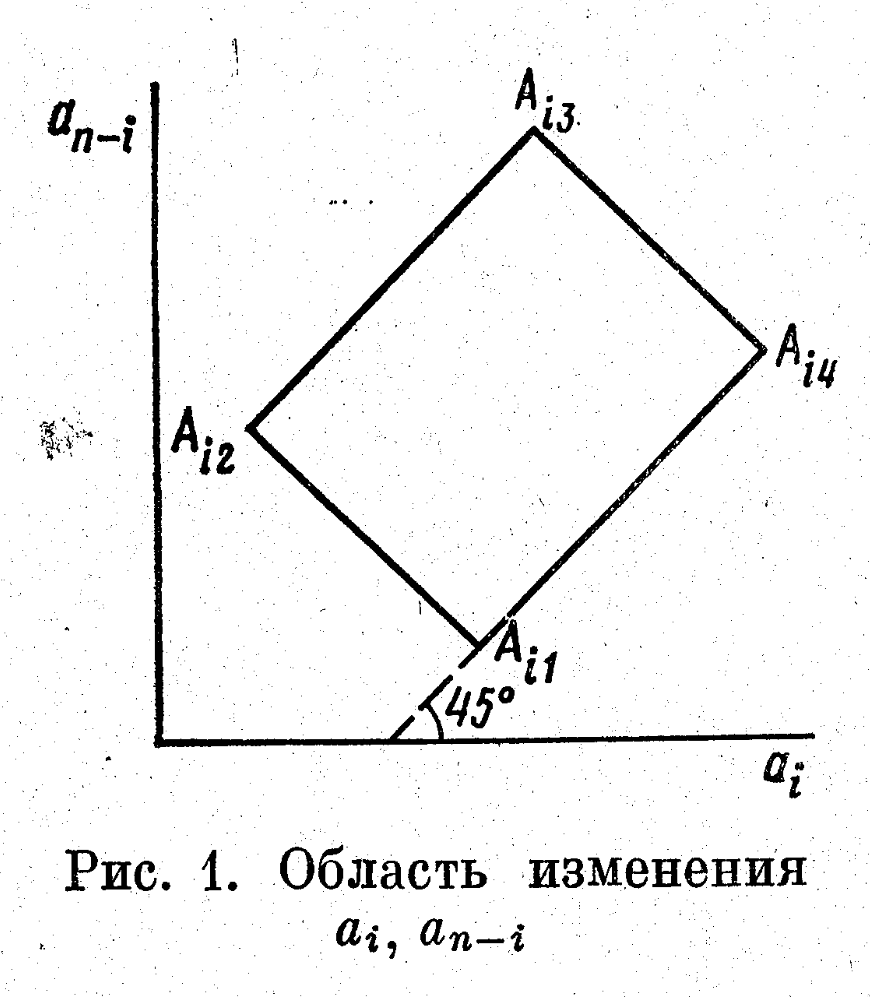
\includegraphics[width=0.27\textwidth]{WeakAnalogue_Area}
    \end{wrapfigure}
    где для всех $i \neq n/2$ $a_i$ и $a_{n-i}$ изменяются внутри области на рис.~1 (если $n$ чётно, то $a_{n/2} \in [\underline{a}_{n/2}, \overline{a}_{n/2}]$).
    Тогда все многочлены $F(z)$ устойчивы и только тогда, когда устойчивы многочлены, коэффициенты которых являются всевозможными
    комбинациями угловых точек (и граничных точек отрезка в случае $i = n/2$).
  \end{theorem}

  \begin{remark}
    Всего таких точек $2^{n+1}$.
  \end{remark}
\end{frame}

\begin{frame}{Достаточное условие как следствие}
  \begin{center}
    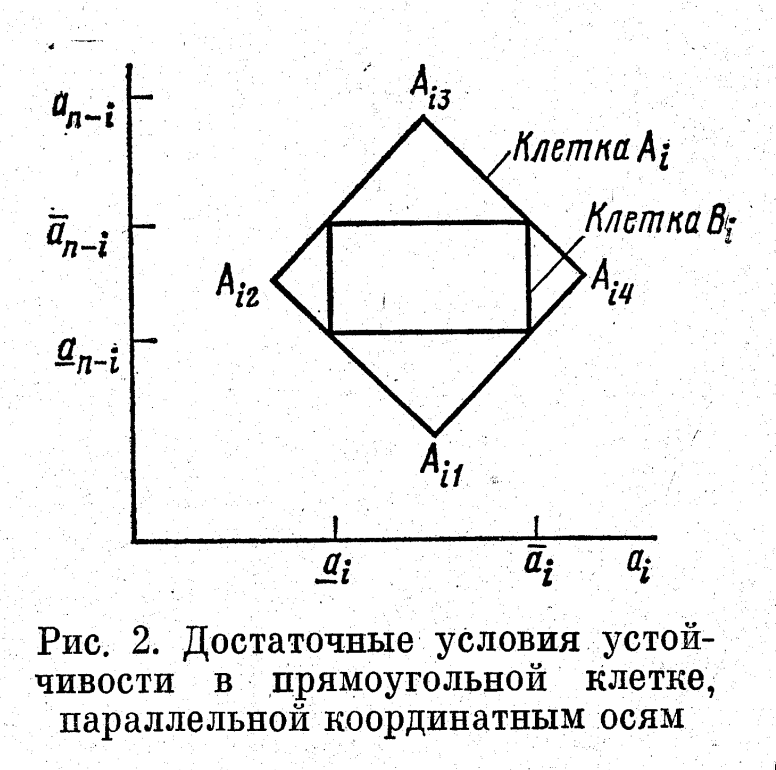
\includegraphics[width=7cm]{WeakAnalogue_SufficientArea}
  \end{center}
\end{frame}

\section{Другой подход к получению достаточных условий}

\begin{frame}{Другой подход: теорема 1}
  Рассмотрим $F_n(s) = a_0s^n + a_1s^{n-1} + \cdots + a_n,\;a_i > 0, \; i=\overline{0,n}$; введём систему параметров
  \begin{equation*}
    \lambda_i = \frac{a_{i-1}a_{i+2}}{a_i a_{i+1}}, \quad i=\overline{1,n-2}, \; n \geqslant 3.
  \end{equation*}

  \begin{theorem}[\cite{LipatovSokolov1978}]\label{th:helper_1}
    Если для некоторого $i \in [1, n-2]$ выполняется условие $\lambda_i > 1$, то система с характеристическим полиномом $F_n(s)$ неустойчива.
  \end{theorem}
\end{frame}

\begin{frame}{Вспомогательная теорема 1: доказательство}
  Для $n=3$ и $n=4$ утверждение следует из критерия Гурвица. \newline

  Предположим, что для устойчивого полинома $F_n(s)$ выполнено $\lambda_i^{(n)} < 1$.
  Покажем, что то же самое верно для устойчивого полинома $F_{n+2}(s)$. \newline

  Пусть $\eta > 0$ и $\mu > 0$ и пусть
  \begin{equation*}
    F_{n+2}(s) = F_n(s) (s^2 + \eta s + \mu) = b_0 s^{n+2} + \cdots + b_{n+2},
  \end{equation*}

  где $b_i = a_{i-2} \mu + a_{i-1} \eta + a_i$ ($a_i = 0$ при $i < 0, i > n$).
\end{frame}

\begin{frame}{Вспомогательная теорема 1: доказательство}
  Для устойчивой системы с полиномом $F_{n+2}(s)$ имеем
  \begin{equation*}
    \begin{aligned}
      b_1 b_{i+1} (1 - \lambda_i^{n+2}) &= b_i b_{i+1} (1 - \frac{b_{i-1} b_{i+2}}{b_{i} b_{i+1}}) \\
      &= (b_i b_{i+1} - b_{i-1} b_{i+2}) \\
      &= \mu^2 (a_{i-2} a_{i-1} - a_{i-3} a_i) + \eta^2 (a_{i-1} a_i - a_{i-2} a_{i+1}) \\
      &\phantom{=\;} + (a_i a_{i+1} - a_{i-1} a_{i+2}) + \eta \mu (a_{i-1}^2 - a_{i-3}a_{i+1}) \\
      &\phantom{=\;} + \eta (a_i^2 - a_{i-2} a_{i+2}) + \mu (a_{i-2} a_{i+1} + a_{i-3} a_{i+2}) \\
      &= \mu^2 a_{i-2} a_{i-1} (1 - \lambda_{i-1}^{(n)}) + \eta^2 a_{i-1} a_i (1 - \lambda_{i-1}^{(n)}) \\
      &\phantom{=\;} + a_i a_{i+1} (1 - \lambda_{i}^{(n)}) + \eta \mu a_{i-1}^2 (1 - \lambda_{i-2}^{(n)} \lambda_{i-1}^{(n)}) \\
      &\phantom{=\;} + \eta a_i^2 (1 - \lambda_{i-1}^{(n)} \lambda_{i}^{(n)}) + \mu a_{i-2} a_{i+3} (1 - \lambda_{i-2}^{(n)} \lambda_{i}^{(n)}).
    \end{aligned}
  \end{equation*}
  Так как по предположению $\eta > 0, \; \mu > 0$ и $\lambda_k^{(n)} < 1$, то все слагаемые в последнем выражении положительны, и, следовательно,
  $\lambda_{i}^{(n+2)} < 1 \quad i=\overline{1,n}$.
\end{frame}

\begin{frame}{Вспомогательная теорема 2}
  \begin{theorem}[\cite{LipatovSokolov1978}]\label{th:helper_2}
    Если для некоторого $i \in [2, n-2]$ выполняется условие $\lambda_{i-1} \lambda_i > C_{ni}$, где
    \begin{equation*}
      \begin{aligned}
        C_{ni} &= \paren{n - i + \frac{{(-1)}^{n+1} - 1}{2}} \paren{i + \frac{{(-1)}^i - 1}{2}} \times \\
        &\times \paren{n - i + \frac{{(-1)}^{n+i} + 3}{2}}^{-1} \paren{i + \frac{{(-1)}^{i} + 3}{2}}^{-1},
      \end{aligned}
    \end{equation*}
    то система с характеристическим полиномом неустойчива.
  \end{theorem}
\end{frame}

\begin{frame}{Вспомогательная теорема 3}
  Образуем из коэффициентов полинома $F_n(s)$ $n-4$ полиномов 5-го порядка:
  \begin{equation}\label{eq:sys_of_poly_5}
    F_{5i} = a_i s^5 + a_{i+1} s^4 + \cdots + a_{i+5}, \quad i=\overline{0,n-5},\; n \geqslant 5.
  \end{equation}

  \begin{theorem}[\cite{LipatovSokolov1978}]
    Пусть корни всех полиномов~\eqref{eq:sys_of_poly_5} расположены в левой полуплоскости.
    Пусть $\lambda_1 + \lambda_2 < 1$ и $\lambda_{n-3} + \lambda_{n-2} < 1$. Тогда система с характеристическим полиномом
    $F_n(s)$ устойчива.
  \end{theorem}

  Доказательство можно найти в~\cite[стр.~34]{LipatovSokolov1978}.
\end{frame}

\begin{frame}{Дальнейшие упрощения}
  \begin{remark}
    В параметрах $\lambda_i$ условия устойчивости для полиномов~\eqref{eq:sys_of_poly_5} выглядят следующим образом:
    \begin{equation}
      \begin{aligned}
        \lambda_{i+1} &< 1 \\
        \lambda_{i+2} &< \frac{(1 - \lambda_{i+1}) (1 - \lambda_{i+3})}{{(1 - \lambda_{i+1}\lambda_{i+3})^2}}, \quad i=\overline{0,n-5}.
      \end{aligned}
    \end{equation}
  \end{remark}
\end{frame}

\begin{frame}{Дальнейшие упрощения: следствия}
  \begin{corollary}[1]
    Пусть для коэффициентов полинома $F_n(s)$ выполняется
    \begin{equation*}
        \lambda_i < \lambda^*, \quad i=\overline{1,n-2}, \; n \geqslant 5,
    \end{equation*}
    где $\lambda^*$ --- вещественный корень уравнения $\lambda {(\lambda + 1)}^2 = 1$ ($\lambda^* \approx 0.465$).
    Тогда система с характеристическим полиномом $F_n(s)$ устойчива.
  \end{corollary}

  \begin{corollary}[2]
    Пусть для коэффициентов полинома $F_n(s)$ выполняется
    \begin{equation*}
        \lambda_i + \lambda_{i+1} < \lambda^{**}, \quad i=\overline{1,n-3}, \; n \geqslant 5,
    \end{equation*}
    где $\lambda^{**} = \dfrac{3}{\sqrt[3]{4}} - 1 \approx 0.89$.
    Тогда система с характеристическим полиномом $F_n(s)$ устойчива.
  \end{corollary}
\end{frame}

\begin{frame}{Пример 1 (\cite{LipatovSokolov1978})}
  Проверить на устойчивость системы с характеристическим полиномом
  \begin{equation*}
    F_7(s) = \frac{s^7}{10^6} + \frac{2 s^6}{10^5} + \frac{6 s^5}{10^4} + \frac{5 s^4}{10^3} + \frac{s^3}{10^2} + \frac{8 s^2}{10} + 7s + 50.
  \end{equation*}

  \begin{solution}
    Вычислим значения $\lambda_i$:~$\lambda_1 = 0.417;\;\lambda_2 = 0.067;\;\lambda_3 = 9.63; \dots$ Так как $\lambda_3 > 1$, то по
    вспомогательной теореме~1 система неустойчива.
  \end{solution}
\end{frame}

\begin{frame}{Пример 2 (\cite{LipatovSokolov1978})}
  Проверить на устойчивость системы с характеристическим полиномом
  \begin{equation*}
    F_6(s) = \frac{s^6}{10^5} + \frac{4 s^5}{10^4} + \frac{15 s^4}{10^3} + \frac{12 s^3}{10^2} + \frac{5 s^3}{10} + 2s + 1,7.
  \end{equation*}

  \begin{solution}
    Вычислим значения $\lambda_i$:~$\lambda_1 = 0.2;$ $\lambda_2 = 0.111;$ $\lambda_3 = 0.5;$ $\lambda_4 = 0.204$. Вспомогательная теорема~1 и следствие~1 неприменимы,
    считаем суммы соседних $\lambda_i$: $\lambda_1 + \lambda_2 = 0.311;$ $\lambda_2 + \lambda_3 = 0.611;$ $\lambda_3 + \lambda_4 = 0.704$. Суммы меньше $0.89$,
    поэтому по следствию~2 система устойчива.
  \end{solution}
\end{frame}

\begin{frame}{Пример 3 (\cite{LipatovSokolov1978})}
  Пусть дан характеристический полином системы
  \begin{equation*}
    F_6(s) = s^6 + 12 s^5 + 47 s^4 + 108 s^3 + 122 s^2 + a_5 s + a_6,
  \end{equation*}
  где параметры $a_5, a_6$ являются искомыми, и требуется найти ``приближённые'' области устойчивости в пространстве
  этих параметров и сравнить их с точной областью устойчивости.

  \begin{solution}
    Проверяем выполнение достаточных условий для коэффициентов, заданных в численном виде:
    \begin{equation*}
      \begin{gathered}
        \lambda_1 \approx 0.19 < 0.465, \\
        \lambda_2 \approx 0.29 < 0.465.
      \end{gathered}
    \end{equation*}
  \end{solution}
\end{frame}

\begin{frame}{Пример 3: необходимые условия}
  Необходимые условия устойчивости вспомогательных теорем 1 и 2 и условия $a_i > 0, \quad i=\overline{0,n}$ накладывают
  на параметры $a_5$ и $a_6$ следующие ограничения:
  \begin{equation*}
    \begin{gathered}
      0 < a_6 < 105, \\
      0.89 a_6 < a_5 < 242.
    \end{gathered}
  \end{equation*}

  Замечание: эти условия являются необходимыми, но не достаточными для устойчивости.
\end{frame}

\begin{frame}{Пример 3: достаточные условия}
  Условия следствия~1 и требование положительности коэффициентов накладывают на параметры следующие ограничения:
  \begin{equation*}
    \begin{gathered}
      0 < a_6 < 0.52 a_5, \\
      a_5 < 130.
    \end{gathered}
  \end{equation*}

  И, наконец, выполнение условия следствия~2 дают следующие неравенства:
  \begin{equation*}
    \begin{gathered}
      0 < a_6 < a_5 - 0.004 a_5^2, \\
      a_5 < 169.
    \end{gathered}
  \end{equation*}

  Замечание: выполнения этих неравенств достаточно для устойчивости системы.
\end{frame}

\begin{frame}{Пример 3: наглядное сравнение}
  \begin{center}
    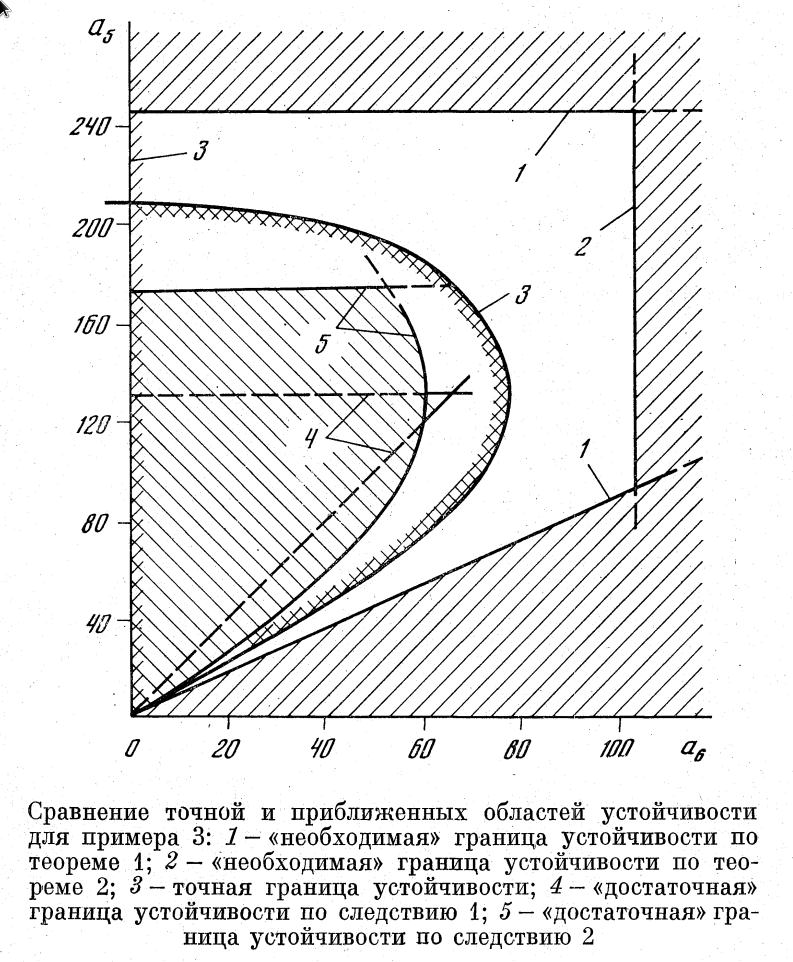
\includegraphics[width=6cm]{Example3_Areas}
  \end{center}
\end{frame}

\begin{frame}{Достаточное условие устойчивости интервального полинома}
  Рассмотрим полином
  \begin{equation}
    F(s) = \sum_{k=0}^n a_k s^{n-k}, \quad a_k \in [x_k, y_k], \quad y_k \geqq x_k > 0, \quad k = \overline{0,n}.
  \end{equation}

  \begin{theorem}
    Интервальный полином $F(s)$ гурвицев, если выполнены $n-2$ соотношения
    \begin{equation}\label{eq:magic_number}
      y_{i-1} y_{i+2} \leqq 0.4655 x_i x_{i+1}, \quad i = \overline{1,n-2}.
    \end{equation}
  \end{theorem}

  \begin{proof}
    Выполнение условия~\eqref{eq:magic_number} гарантирует, что для любого фиксированного $a_k \in [x_k, y_k], \quad k = \overline{0,n}$ полином $F(s)$ гурвицев.
  \end{proof}
\end{frame}

\begin{frame}[shrink=35]{Литература}
  \nocite{Jury1990Ru}
  \printbibliography{}
  Полный список: \url{https://uni.sharshukov.xyz/bib}.

  Исходный код:
  \href{https://github.com/arealhero/uni/blob/master/Latex/Presentations/DiscreteRobustness/DiscreteRobustness.tex}{\texttt{https://github.com/arealhero/uni}}.
\end{frame}

\end{document}
